\documentclass[10pt,a4paper]{article}
\usepackage[utf8]{inputenc}
\usepackage[francais]{babel}
\usepackage[T1]{fontenc}
\usepackage{amsmath}
\usepackage{amsfonts}
\usepackage{amssymb}
\usepackage{graphicx}
\usepackage[a4paper]{geometry}
\setlength{\oddsidemargin}{0pt} % Marge gauche sur pages impaires
\setlength{\evensidemargin}{9pt} % Marge gauche sur pages paires
\setlength{\marginparwidth}{54pt} % Largeur de note dans la marge
\setlength{\textwidth}{481pt} % Largeur de la zone de texte (17cm)
\setlength{\voffset}{-18pt} % Bon pour DOS
\setlength{\marginparsep}{7pt} % Séparation de la marge
\setlength{\topmargin}{0pt} % Pas de marge en haut
\setlength{\headheight}{13pt} % Haut de page
\setlength{\headsep}{10pt} % Entre le haut de page et le texte
\setlength{\footskip}{27pt} % Bas de page + séparation
\setlength{\textheight}{708pt} % Hauteur de la zone de texte (25cm)

\title{Réalisation des processeurs Nono-1 et Nono-2 \\ \textit{Projet d'Architecture des ordinateurs}}
\author{Florian Delavernhe et Thomas Minier \\ groupe 501A}
\date{18 Décembre 2014}
\begin{document}

\maketitle
\vspace{3cm}
\tableofcontents
\newpage

\section{Introduction}

Dans le cadre de ce projet, il nous a été demandé de réaliser un processeur Nono-1 à 16 registres. Il supporte jusqu'à 16 instructions différentes, réparties sur trois formats de données.

Nous avons utilisé le logiciel \textit{Logisim} pour modéliser le circuit et les programmes de tests ont été écrits en assembleur et en binaire.

\section{Implémentation du Nono-1}

\subsection{Unité arithmétique logique}

Pour réaliser cette UAL , nous avons décidé d'effectuer chacune des opérations possibles en fonction des deux entrées, puis de diriger les résultats de chacune de ces opérations dans un multiplexeur. En fonction du code sur l'entrée \textit{ctrlUAL}, nous envoyons dans la sortie le résultat correspondant à l'opération souhaitée. Le code reçu par le multiplexeur est détaillé dans la Figure \ref{code_ctrlUAL}. 
Concernant les différents flags, nous rappelons leur signification et comment nous avons choisi de les implémenter :
\begin{itemize}
\item \textbf{CF}, ou \textit{Carry Flag}, est armé si une opération arithmétique génère une retenue. Pour l'implémenter, nous identifions d'abord quelles sont les opérations susceptibles de générer une retenue : l'addition et la soustraction. Nous faisons alors un test logique \verb|OU| sur les sorties des retenues de ces deux opérations. Si l'une d'elles est vraie, alors il y a bien une retenue et le \textit{Carry Flag} est armé.
\item \textbf{ZF}, ou \textit{Zero Flag}, est armé si le résultat d'une opération arithmétique est égal à zéro. Pour l'implémenter, nous faisons simplement un test logique \verb|ET| entre la sortie de l'UAL et une constante fixée à \verb|00000000|, ce qui revient à tester si la sortie est égal à zéro codé sur 8 bits. Si le test vaut vrai, alors le \textit{Zero Flag} est armé.
\item \textbf{SF}, ou \textit{Sign Flag}, est armé si le résultat d'une opération arithmétique possède un bit de poids fort à 1, signalant ainsi un résultat signé. Pour l'implémenter, nous récupérons le bit de pids fort du résultat avec un splitter, puis nous testons avec un \verb|ET| s'il est égal à 1. Si le test vaut vrai, alors le \textit{Sign Flag} est armé.
\item \textbf{OF}, ou \textit{Overflow Flag}, est armé si le résultat constitue un nombre dont le codage dépasse 8 bits. Pour l'implémenter, nous faisons un test logique \verb|ET| entre les deux bits de poids forts des entrées. Si le test est vrai, alors le \textbf{OF} est armé.
\end{itemize} 

Une fois ces 4 drapeaux identifiés et armés s'il le faut, nous concaténons leurs valeurs au moyen d'un splitter (dans l'ordre \textbf{CF - ZF - SF - OF}) puis nous envoyons ce nombre sur 4 bits dans la sortie \textit{flags} de l'UAL. \\
Le détail du circuit de l'UAL se trouve dans les annexes à la Figure \ref{circuit_ual}.

\subsection{Décodeur d'instruction}

Pour implémenter le décodeur d'instructions, nous codons les différentes opérations comme indiqué dans la Figure \ref{codage_instructions}.

Nous avons choisi ce codage précis pour nous permettre de réduire le circuit logique. En effet, nous avons fait en sorte que toutes les instructions de saut aient leur 3ème bit égal à 1. Les autres instructions elles ont leur 3ème bit égal à zéro. \\

Pour les instructions de saut, nous allons avoir besoin que l'UAl effectue une soustraction. Pour ce faire, nous relions la sortie du décodeur à un multiplexeur. Si \text{isJUmp} est vrai, alors nous renvoyons le code \verb|0 0 1|, qui correspond à l'instruction sub. Sinon, nous renvoyons le code sans son 3ème bit, qui est inutile. \\

Pour armer ou non les drapeaux \textit{isLoad}, \textit{regWrite} et \textit{isJMP}, nous dressons les tableaux de Karnaugh des Figures \ref{karnaugh_isload}, \ref{karnaugh_regwrite} et \ref{karnaugh_isjmp}.

On en déduit que $isLoad = A~\overline{B}~C~D$, $regWrite = \overline{B}$ et $isJMP = B$. Le détail du circuit se trouve dans la Figure \ref{circuit_decodeur}. \newpage

\subsection{Contrôle de saut}

Ce module envoyant dans sa sortie un code sur 2 bits indiquant quel type de saut il faut faire (instruction suivante, HALT ou saut), nous commençons par établir le codage de cette sortie, indiqué dans la Figure \ref{code_sortie_controle}. L'entrée correspond au code \verb|1 0| au niveau du multiplexeur en sortie du module sera neutralisée.

En reprenant notre codage des différentes instructions, nous remarquons qu'il est possible de simplifier une fois encore le circuit. En effet, si le 3ème bit du code est égal à 0, alors $e_0 = 0$. Sinon, $e_0 = 1$. Nous pouvons donc donc déterminer facilement la valeur de $e_0$ avec un simple test logique \verb|ET| entre le troisième bit du code et une constante fixée à \verb|0|. \\

Ensuite, nous nous intéressons à $e_1$. Pour pouvoir implémenter le module, nous devons pouvoir effectuer les tests liés aux différentes instructions de saut conditionnelle. Nous avons donc remarqué les analogies suivantes :
\begin{itemize}
\item L'instruction \textbf{beq, \$t0, \$t1, etq} peut se traduire par : si $\$t0 - \$t1 = 0$, alors on saute à $etq$.
\item L'instruction \textbf{bne, \$t0, \$t1, etq} peut se traduire par : si $\$t0 - \$t1\neq0$, alors on saute à $etq$.
\item L'instruction \textbf{bge, \$t0, \$t1, etq} peut se traduire par : si $\$t0 - \$t1 \geq0$, alors on saute à $etq$.
\item L'instruction \textbf{ble, \$t0, \$t1, etq} peut se traduire par : si $\$t0 - \$t1 \leq0$, alors on saute à $etq$.
\item L'instruction \textbf{bgt, \$t0, \$t1, etq} peut se traduire par : si $\$t0 - \$t1 > 0$, alors on saute à $etq$.
\item L'instruction \textbf{blt, \$t0, \$t1, etq} peut se traduire par : si $\$t0 - \$t1 < 0$, alors on saute à $etq$.
\item L'instruction \textbf{b etq} ne nécessite aucune interprétation, on saute à $etq$ dès que cette instruction est lue.
\item Même chose pour l'instruction \textbf{halt}. On arrête le programme dès qu'elle est lue.
\end{itemize}
\vspace{0.2cm}
Pour les instructions \textbf{beq} et \textbf{bne}, il nous faudra donc regarder si le drapeau \textbf{ZF} est armé ou non. Pour les autres instructions, il nous faudra regarder les drapeaux \textbf{ZF} et \textbf{SF}. Nous établissons donc une table de vérité, directement exprimée sous la forme d'un tableau de Karnaugh et détaillée dans la Figure \ref{karnaugh_controle}

On en déduit que $e_1 = \overline{A}~\overline{C}~D + \overline{A}~D~\overline{ZF}~\overline{SF} + \overline{A}~C~\overline{D}~ZF + A~C~\overline{D}~\overline{SF} + A~D~\overline{ZF}~SF + \overline{C}~\overline{ZF}~\overline{SF} + A$. Le détail du circuit se trouve à la Figure \ref{circuit_controle}.

\subsection{Banc de registres}

Nous commençons par coder la sélection de registres avec rd, rs et rt, détaillé dans la Figure \ref{code_registres}. Ensuite, nous réalisons un sous-circuit \textbf{décodeur rd} qui se charge, en fonction du code de l'entrée, de faire sortir 1 sur la sortie correspondant au registre que l'on veut sélectionner. Les autres sorties sont mises à 0. 

Grâce à ce sous-circuit, nous pouvons réaliser le module. Nous faisons rentrer \textit{valin} dans l'entrée de chaque registre. Pour savoir s'il faut écrire ou non dans un registre, nous faisons un test logique \verb|ET| entre la sortie de \textbf{decodeur rd}, qui correspond au registre courant, et \textit{regWrite}. Le résultat de ce test est alors envoyé dans le verrou du registre courant.

Enfin, nous utilisons des multiplexeurs pour déterminer les sorties du module. Les sorties de chaque registre sont envoyées dans chacun des multiplexeurs et les valeurs de \textit{rs} et \textit{rt} servent à sélectionner les bonnes valeurs qui seront envoyées dans les sorties. Le détail du circuit se trouve à la Figure \ref{circuit_banc}. 

\subsection{Sélection de registres}

Pour ce module, nous avons simplement à vérifier la valeur de \textit{isJMP}. Si elle vaut 1, alors on a les sorties suivantes :
\begin{itemize}
\item \textit{rd} = \{rd/rs\}
\item \textit{rs} = \{rs/rt\}
\item \textit{rt} = \{rt\}
\end{itemize}
Sinon, alors on a les sorties suivantes :
\begin{itemize}
\item \textit{rd} = \{rd/rs\}
\item \textit{rs} = \{rd/rs\}
\item \textit{rt} = \{rs/rt\}
\end{itemize}
Le détail du circuit se trouve à la Figure \ref{circuit_selection}.
\newpage
\section{Utilisation du Nono-1}

\subsection{Implémentation de l'instruction halt}

D'après la figure de l'énoncé, l'instruction \textit{halt} est implémentée par une constante qui déclenche un saut à la fin du programme.

Cela impose une contrainte sur le code machine. En effet, étant donné que la constante \textit{halt} vaut \verb|0xFF|, on ne peut pas avoir d'instructions au delà de cette adresse. Sinon, l'instruction halt représenterait un simple saut et non la fin du programme.

\subsection{Fonction pgcd}

Le code assembleur et binaire se trouve dans les fichiers \textbf{bin/pgcd.asm} et \textbf{bin/pgcd.bin}.

\subsection{Fonction pow}

Nous avons décidé de coder la fonction puissance, qui renvoie $2^i$, où $i$ est précisé dans le programme. Le code assembleur et binaire se trouve dans les fichiers \textbf{bin/pow.asm} et \textbf{bin/pow.bin}.

\subsection{Processeur Nono-2}

Nous n'avons pas eu le temps de traiter la question, par manque de temps.

\section{Conclusion}

En conclusion, ce projet aura été assez intéressant. Il nous aura permis de comprendre le fonctionnement d'un processeur et comment le code assembleur est interprété et utilisé par le circuit.

\section{Annexes}

\begin{figure}[h]
\centering
\begin{tabular}{|c|c|}
 \hline
 \textbf{Instruction} & \textbf{code} \\
 \hline
 add & \verb|0 0 0| \\
 \hline
 sub & \verb|0 0 1| \\
 \hline
 or & \verb|0 1 0| \\
 \hline
 and & \verb|0 1 1| \\
 \hline
 not & \verb|1 0 0| \\
 \hline
 right shift & \verb|1 0 1| \\
 \hline
 left shift & \verb|1 1 0| \\
 \hline
\end{tabular}
\caption{Codage de ctrlUAL}
\label{code_ctrlUAL}
\end{figure}

\begin{figure}[h]
\centering
\begin{tabular}{|c|c|}
 \hline
 \textbf{Instruction} & \textbf{A B C D} \\
 \hline
 add & \verb|0 0 0 0| \\
 \hline
 sub & \verb|0 0 0 1| \\
 \hline
 or & \verb|0 0 1 0| \\
 \hline
 and & \verb|0 0 1 1| \\
 \hline
 halt & \verb|0 1 0 0| \\
 \hline
 b & \verb|0 1 0 1| \\
 \hline
 beq & \verb|0 1 1 0| \\
 \hline
 bne & \verb|0 1 1 1| \\
 \hline
 not & \verb|1 0 0 0| \\
 \hline
 shl & \verb|1 0 0 1| \\
 \hline
 shr & \verb|1 0 1 0| \\
 \hline
 li & \verb|1 0 1 1| \\
 \hline
 bge & \verb|1 1 0 0| \\
 \hline
 ble & \verb|1 1 0 1| \\
 \hline
 bgt & \verb|1 1 1 0| \\
 \hline
 blt & \verb|1 1 1 1| \\
 \hline
\end{tabular}
\caption{Codage des instructions sur 4 bits}
\label{codage_instructions}
\end{figure}

\begin{figure}[h]
\centering
\begin{tabular}{|c|c|c|c|c|}
 \hline
 \textbf{$A B \backslash C D$} & \verb|0 0| & \verb|0 1| & \verb|1 1| & \verb|1 0|\\
 \hline
  \verb|0 0| & \verb|0| & \verb|0| & \verb|0| & \verb|0| \\
 \hline
   \verb|0 1| & \verb|0| & \verb|0| & \verb|0| & \verb|0| \\
 \hline
   \verb|1 1| & \verb|0| & \verb|0| & \verb|0| & \verb|0| \\
 \hline
   \verb|1 0| & \verb|0| & \verb|0| & \verb|1| & \verb|0| \\
 \hline
\end{tabular}
\caption{Tableau de Karnaugh de isLoad}
\label{karnaugh_isload}
\end{figure}

\begin{figure}[h]
\centering
\begin{tabular}{|c|c|c|c|c|}
 \hline
 \textbf{$A B \backslash C D$} & \verb|0 0| & \verb|0 1| & \verb|1 1| & \verb|1 0|\\
 \hline
  \verb|0 0| & \verb|1| & \verb|1| & \verb|1| & \verb|1| \\
 \hline
   \verb|0 1| & \verb|0| & \verb|0| & \verb|0| & \verb|0| \\
 \hline
   \verb|1 1| & \verb|0| & \verb|0| & \verb|0| & \verb|0| \\
 \hline
   \verb|1 0| & \verb|1| & \verb|1| & \verb|1| & \verb|1| \\
 \hline
\end{tabular}
\caption{Tableau de Karnaugh de regWrite}
\label{karnaugh_regwrite}
\end{figure}

\begin{figure}[h]
\centering
\begin{tabular}{|c|c|c|c|c|}
 \hline
 \textbf{$A B \backslash C D$} & \verb|0 0| & \verb|0 1| & \verb|1 1| & \verb|1 0|\\
 \hline
  \verb|0 0| & \verb|0| & \verb|0| & \verb|0| & \verb|0| \\
 \hline
   \verb|0 1| & \verb|1| & \verb|1| & \verb|1| & \verb|1| \\
 \hline
   \verb|1 1| & \verb|1| & \verb|1| & \verb|1| & \verb|1| \\
 \hline
   \verb|1 0| & \verb|0| & \verb|0| & \verb|0| & \verb|0| \\
 \hline
\end{tabular}
\caption{Tableau de Karnaugh de isJMP}
\label{karnaugh_isjmp}
\end{figure}

\begin{figure}[h]
\centering
\begin{tabular}{|c|c|}
 \hline
 \textbf{Type de saut} & \textbf{$e_1 e_0$} \\
 \hline
 instruction suivante & \verb|0 0| \\
 \hline
  HALT & \verb|0 1| \\
 \hline
  saut & \verb|1 1| \\
 \hline
\end{tabular}
\caption{Codage de la sortie du contrôle de saut}
\label{code_sortie_controle}
\end{figure}

\begin{figure}[h]
\centering
\begin{tabular}{|c|c|c|c|c|c|}
 \hline
 \textbf{Instruction} & \textbf{$A C D \backslash ZF SF$} & \verb|0 0| & \verb|0 1| & \verb|1 1| & \verb|1 0|\\
 \hline
  b & \verb|0 0 1| & \verb|1| & \verb|1| & \verb|1| & \verb|1| \\
 \hline
   bne & \verb|0 1 1| & \verb|1| & \verb|1| & \verb|0| & \verb|0| \\
 \hline
   beq & \verb|0 1 0| & \verb|0| & \verb|0| & \verb|1| & \verb|1| \\
 \hline
   bgt & \verb|1 1 0| & \verb|1| & \verb|0| & \verb|0| & \verb|0| \\
 \hline
   halt & \verb|1 1 1| & \verb|0| & \verb|1| & \verb|0| & \verb|0| \\
 \hline
   ble & \verb|1 0 1| & \verb|0| & \verb|1| & \verb|1| & \verb|1| \\
 \hline
   bge & \verb|1 0 0| & \verb|1| & \verb|0| & \verb|1| & \verb|1| \\
 \hline
\end{tabular}
\caption{Tableau de Karnaugh du contrôle de saut}
\label{karnaugh_controle}
\end{figure}

\begin{figure}[h]
\centering
\begin{tabular}{|c|c|}
 \hline
 \textbf{Registre} & \textbf{A B C D} \\
 \hline
 r0 & \verb|0 0 0 0| \\
 \hline
 r1 & \verb|0 0 0 1| \\
 \hline
 r2 & \verb|0 0 1 0| \\
 \hline
 r3 & \verb|0 0 1 1| \\
 \hline
 r4 & \verb|0 1 0 0| \\
 \hline
 r5 & \verb|0 1 0 1| \\
 \hline
 r6 & \verb|0 1 1 0| \\
 \hline
 r7 & \verb|0 1 1 1| \\
 \hline
 r8 & \verb|1 0 0 0| \\
 \hline
 r9 & \verb|1 0 0 1| \\
 \hline
 r10 & \verb|1 0 1 0| \\
 \hline
 r11 & \verb|1 0 1 1| \\
 \hline
 r12 & \verb|1 1 0 0| \\
 \hline
 r13 & \verb|1 1 0 1| \\
 \hline
 r14 & \verb|1 1 1 0| \\
 \hline
 r15 & \verb|1 1 1 1| \\
 \hline
\end{tabular}
\caption{Codage de la sélection de registres sur 4 bits}
\label{code_registres}
\end{figure}

% UAL
\begin{figure}[h]
\centering
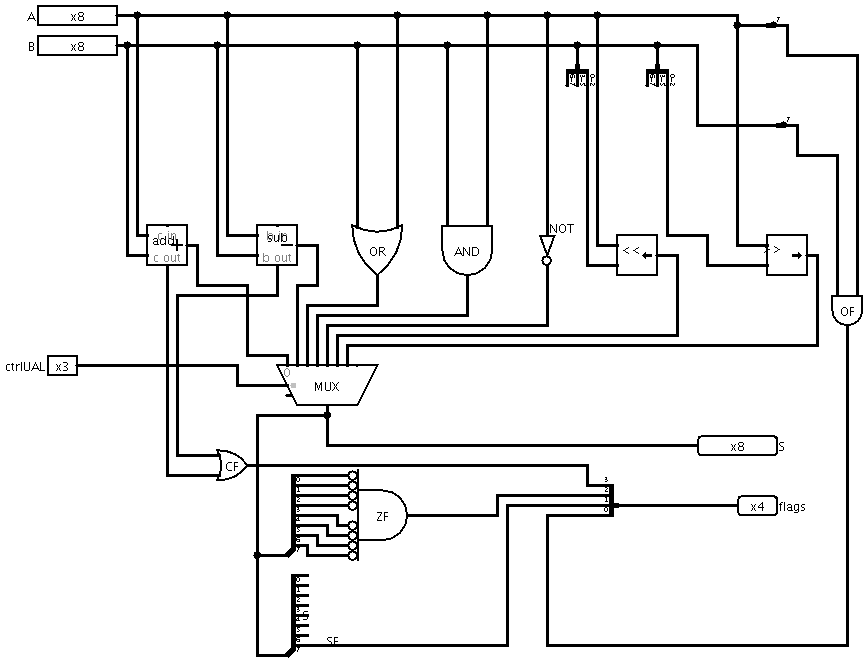
\includegraphics[scale=0.5]{img/UAL.png}
\caption{Circuit logique de l'UAL}
\label{circuit_ual}
\end{figure}

% Décodeur d'instructions
\begin{figure}[h]
\centering
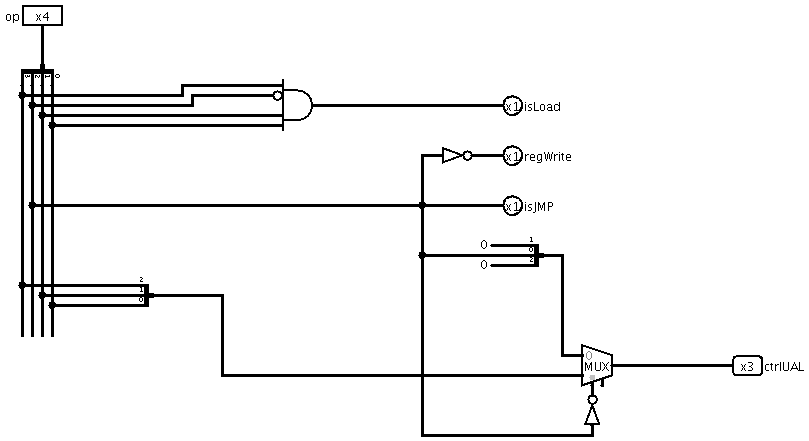
\includegraphics[scale=0.5]{img/decodeur.png}
\caption{Circuit logique du décodeur d'instructions}
\label{circuit_decodeur}
\end{figure}

% Contrôle de saut
\begin{figure}[h]
\centering
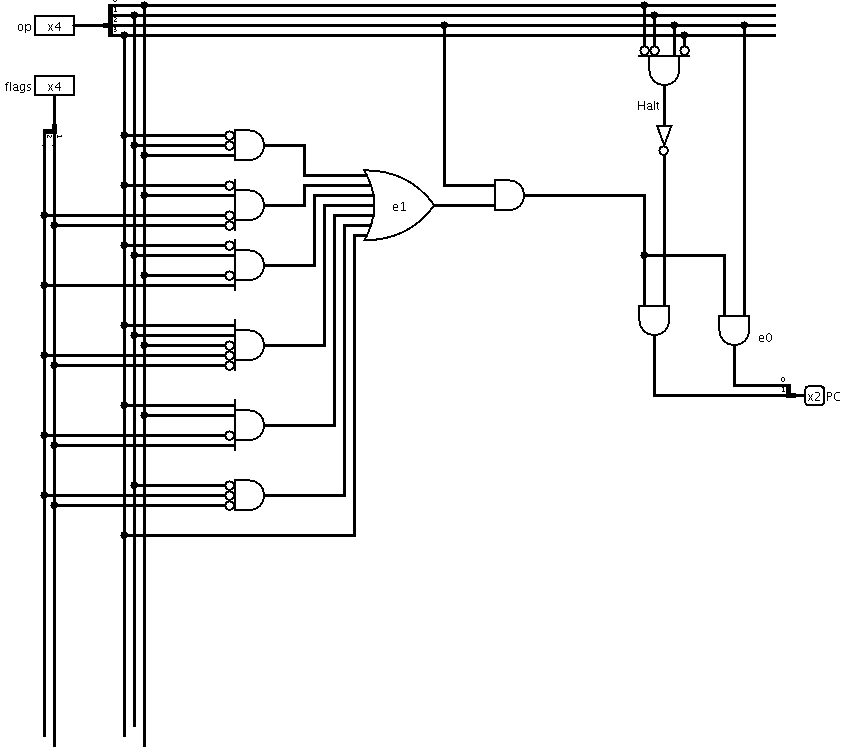
\includegraphics[scale=0.5]{img/controle_saut.png}
\caption{Circuit logique du contrôle de saut}
\label{circuit_controle}
\end{figure}

% Banc de registres
\begin{figure}[h]
\centering
\rotatebox{90}{
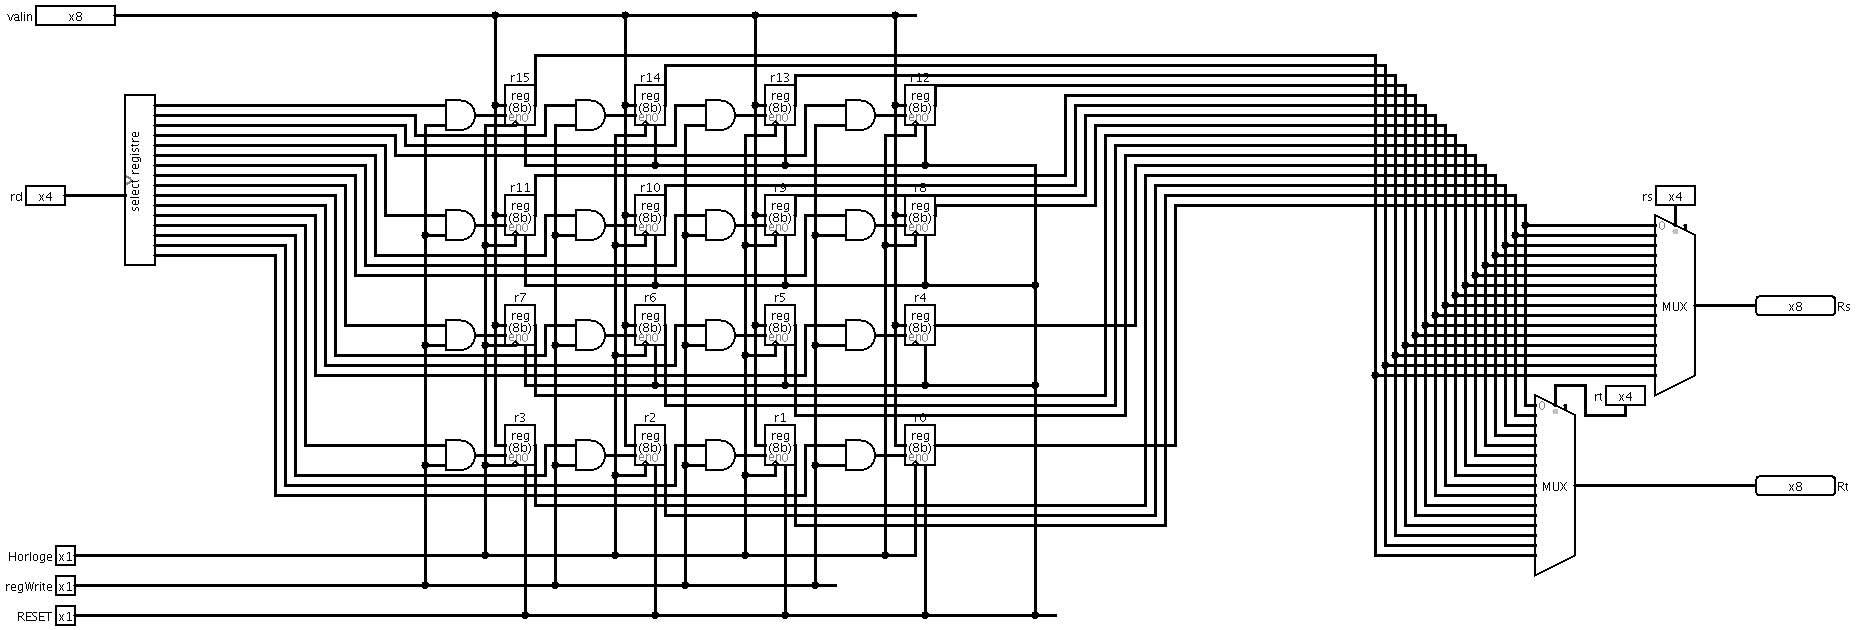
\includegraphics[scale=0.3]{img/banc_registres.png}
}
\caption{Circuit logique du banc de registres}
\label{circuit_banc}
\end{figure}

% Sélection de registres
\begin{figure}[h]
\centering
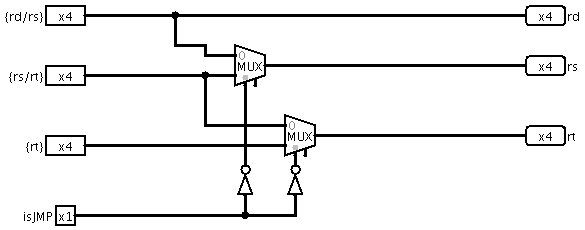
\includegraphics[scale=0.5]{img/selection_registres.png}
\caption{Circuit logique de la sélection de registres}
\label{circuit_selection}
\end{figure}

% Circuit complet
\begin{figure}[h]
\centering
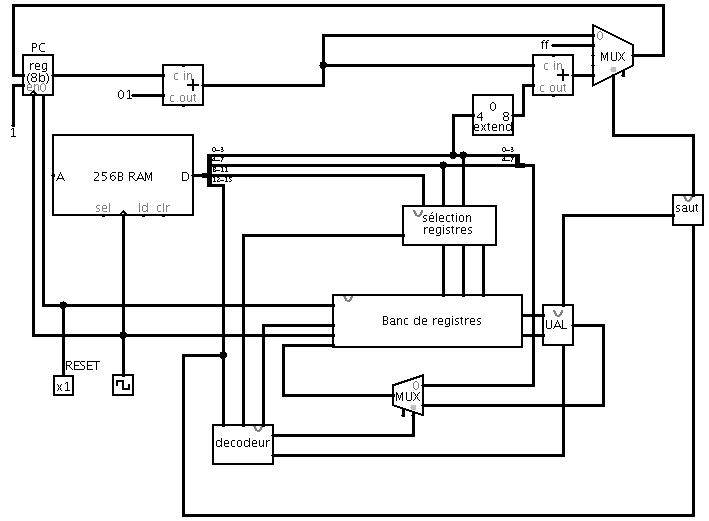
\includegraphics[scale=0.5]{img/Nono.png}
\caption{Circuit du processeur Nono-1}
\label{circuit_nono}
\end{figure}

\end{document}
